\chapter{Working with hyperspectral data}
\label{ch:hyper_basic}


\begin{wrapfigure}{o}{0.5\textwidth}
    \centering
    \vspace{-3cm}
    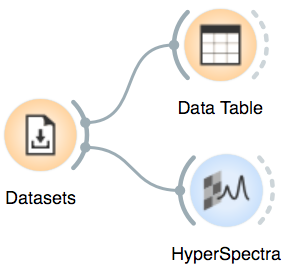
\includegraphics[scale=0.4]{hyperspectral-fig1.png}
    \label{fig:hyper_basic-fig1}
\end{wrapfigure}

We can also visualize hyperspectral data sets. In the \textit{Datasets} widget you will find “Liver cirrhosis” data. Connecting to a \textit{Data Table}, you will see that each spectrum contains information (in meta variables) about image positions (map\_x and map\_y). \mutation\ can recognize the image positioning features from the file automatically. Otherwise, you could set them manually in the image Menu under the \textit{Axis x} and \textit{Axis y} options. 

\begin{figure}[h]
    \centering
    % \vspace{-1cm}
    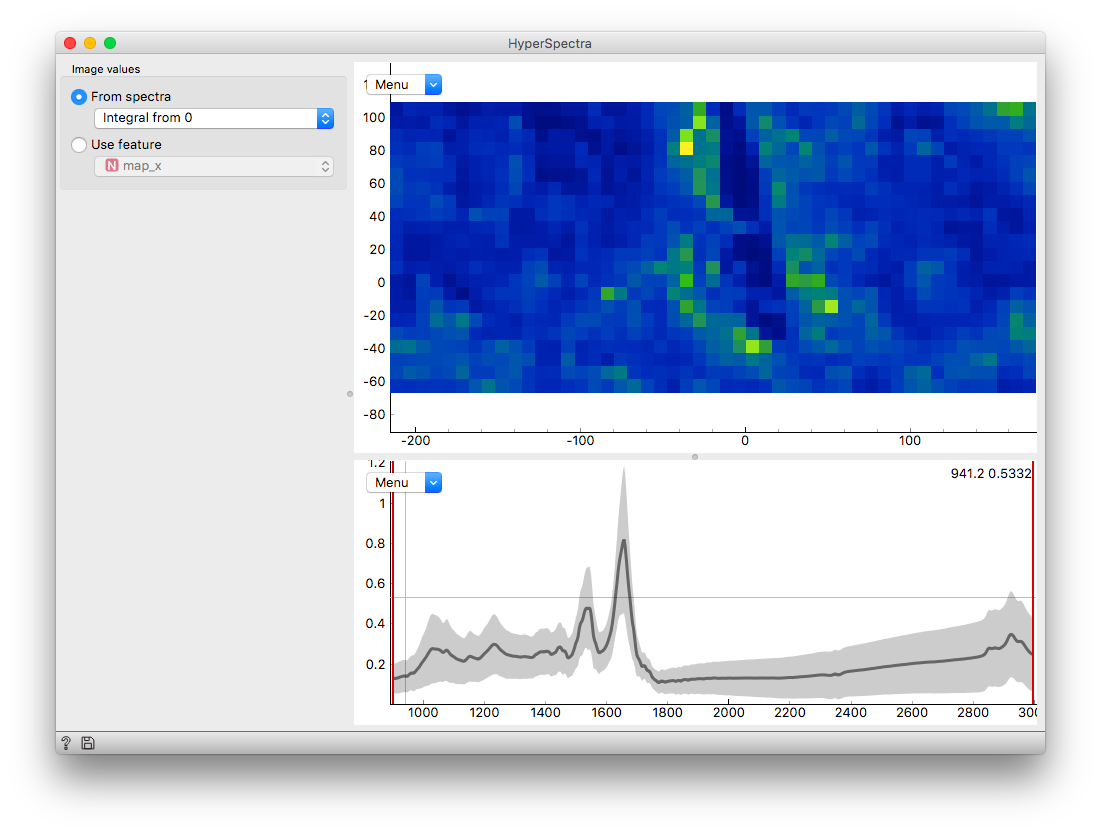
\includegraphics[width=0.8\textwidth]{hyperspectral-fig2.png}
    \caption{The \textit{HyperSpectra} widget has two main parts, it can show image (top) and a spectra (bottom). Explore the options on both plots in their Menus and the left panel, where you can change the visualization parameters.}
    \label{fig:hyper_basic-fig2}
\end{figure}

By default, the image is the 2D representation of the whole integral of each spectrum. To change  it, move the red lines on the spectrum plot. With the dropdown menu on the left panel you can select other representations.

\begin{figure}[h]
    \centering
    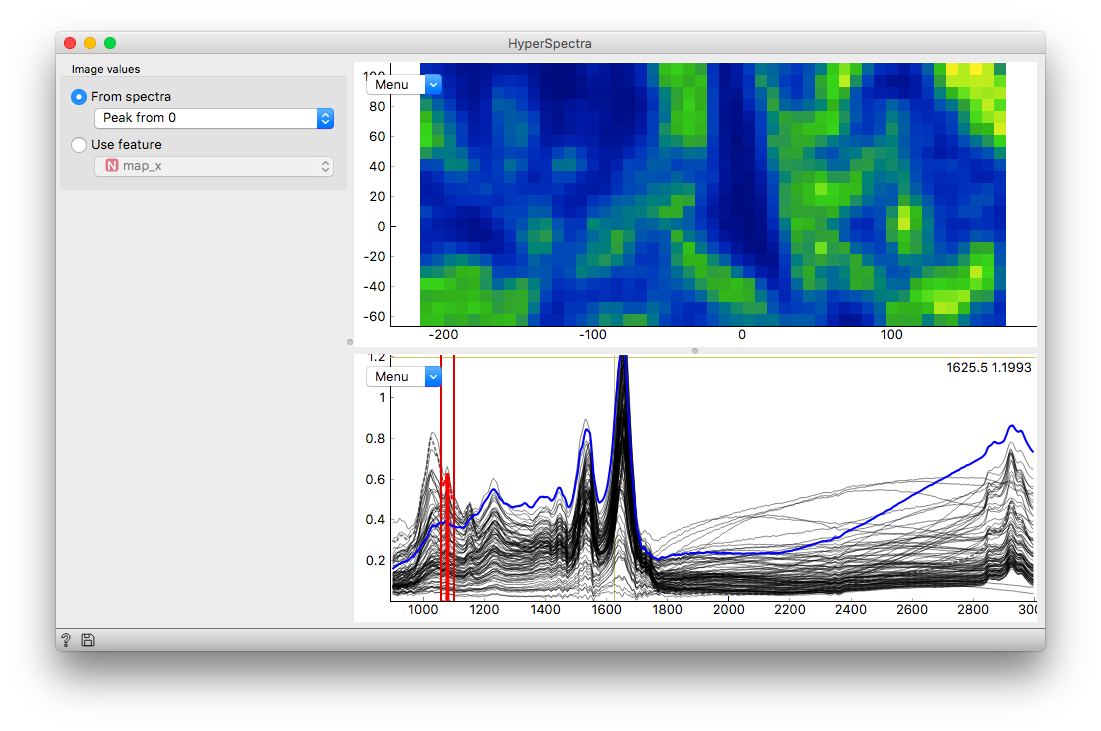
\includegraphics[width=0.8\textwidth]{hyperspectral-fig3.png}
    \caption{To view the plotted integrals, set the spectra display to show individual spectra and click a spectrum. Integrals for the selected spectrum are shaded.}
    \label{fig:hyper_basic-fig3}
\end{figure}
